\documentclass{article}

% if you need to pass options to natbib, use, e.g.:
% \PassOptionsToPackage{numbers, compress}{natbib}
% before loading nips_2018

% ready for submission
\usepackage{nips_2018}

% to compile a preprint version, e.g., for submission to arXiv, add
% add the [preprint] option:
% \usepackage[preprint]{nips_2018}

% to compile a camera-ready version, add the [final] option, e.g.:
% \usepackage[final]{nips_2018}

% to avoid loading the natbib package, add option nonatbib:
% \usepackage[nonatbib]{nips_2018}

\usepackage[utf8]{inputenc} % allow utf-8 input
\usepackage[T1]{fontenc}    % use 8-bit T1 fonts
\usepackage{hyperref}       % hyperlinks
\usepackage{url}            % simple URL typesetting
\usepackage{booktabs}       % professional-quality tables
\usepackage{amsfonts}       % blackboard math symbols
\usepackage{nicefrac}       % compact symbols for 1/2, etc.
\usepackage{microtype}      % microtypography

\usepackage{graphicx}
\usepackage{amsmath}

\title{Classifying Handwritten Digits with a Convolutional Deep Neural Network}

% The \author macro works with any number of authors. There are two
% commands used to separate the names and addresses of multiple
% authors: \And and \AND.
%
% Using \And between authors leaves it to LaTeX to determine where to
% break the lines. Using \AND forces a line break at that point. So,
% if LaTeX puts 3 of 4 authors names on the first line, and the last
% on the second line, try using \AND instead of \And before the third
% author name.

\author{
  Samuel C Williams\\
  South Dakota School of Mines and Technology\\
  Rapid City, SD 57701 \\
  \texttt{samuel.williams@mines.sdsmt.edu} \\
  %% examples of more authors
  %% \And
  %% Coauthor \\
  %% Affiliation \\
  %% Address \\
  %% \texttt{email} \\
  %% \AND
  %% Coauthor \\
  %% Affiliation \\
  %% Address \\
  %% \texttt{email} \\
  %% \And
  %% Coauthor \\
  %% Affiliation \\
  %% Address \\
  %% \texttt{email} \\
  %% \And
  %% Coauthor \\
  %% Affiliation \\
  %% Address \\
  %% \texttt{email} \\
}

\begin{document}
% \nipsfinalcopy is no longer used

\maketitle

\begin{abstract}
  Neural networks excel at solving classification problems. A simple implementation of a deep neural network with convolutional and pooling layers saw success at classifying members of the MNIST dataset: labeled images of handwritten digits.
\end{abstract}

\section{Introduction}

In order to classify the digits in the MNIST dataset, a deep convolutional neural network was used, but what exactly does that mean? The network contained convolutional, pooling, and fully connected layers, each serving either to increase efficiency of training or accuracy of classification. Training was performed on randomly selected batches of 100 digits. 5000 of these batches were used for training. This process was repeated twice more in order to achieve a clearer idea of the networks performance.

\section{The MNIST Dataset}

The MNIST dataset consists of 70,000 images of handwritten digits, and labels defining which digit they represent. There are 60,000 in the training set, and 10,000 in the testing set. Each image has a height and width of 28 pixels on a single black/white color channel. See figure 1.

\begin{figure}
  \centering
  	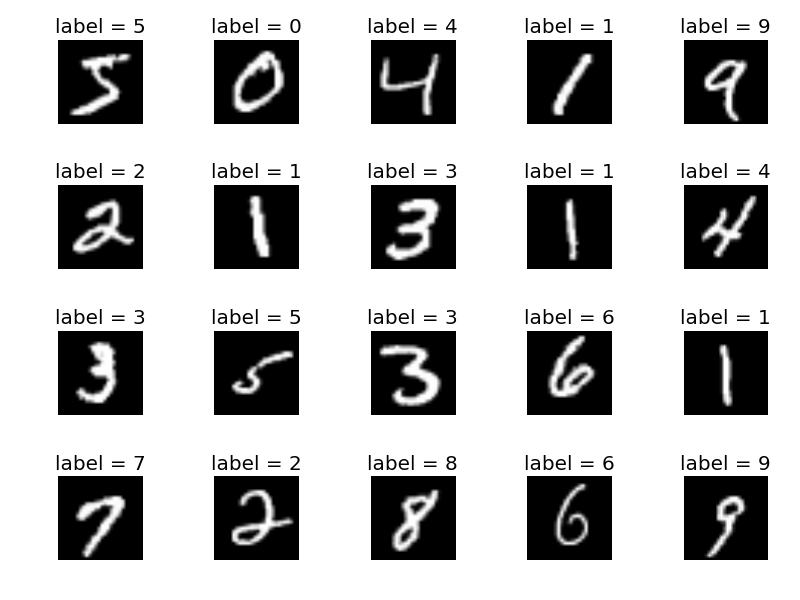
\includegraphics[width=0.8\linewidth]{figures/mnist_example}
  \caption{Sample images for the MNIST dataset.}
\end{figure}

\section{Network Structure}

The network consisted of of two convolutional layers, two pooling layers, and one fully connected layer. See figure 2.

\begin{figure}
  \centering
  	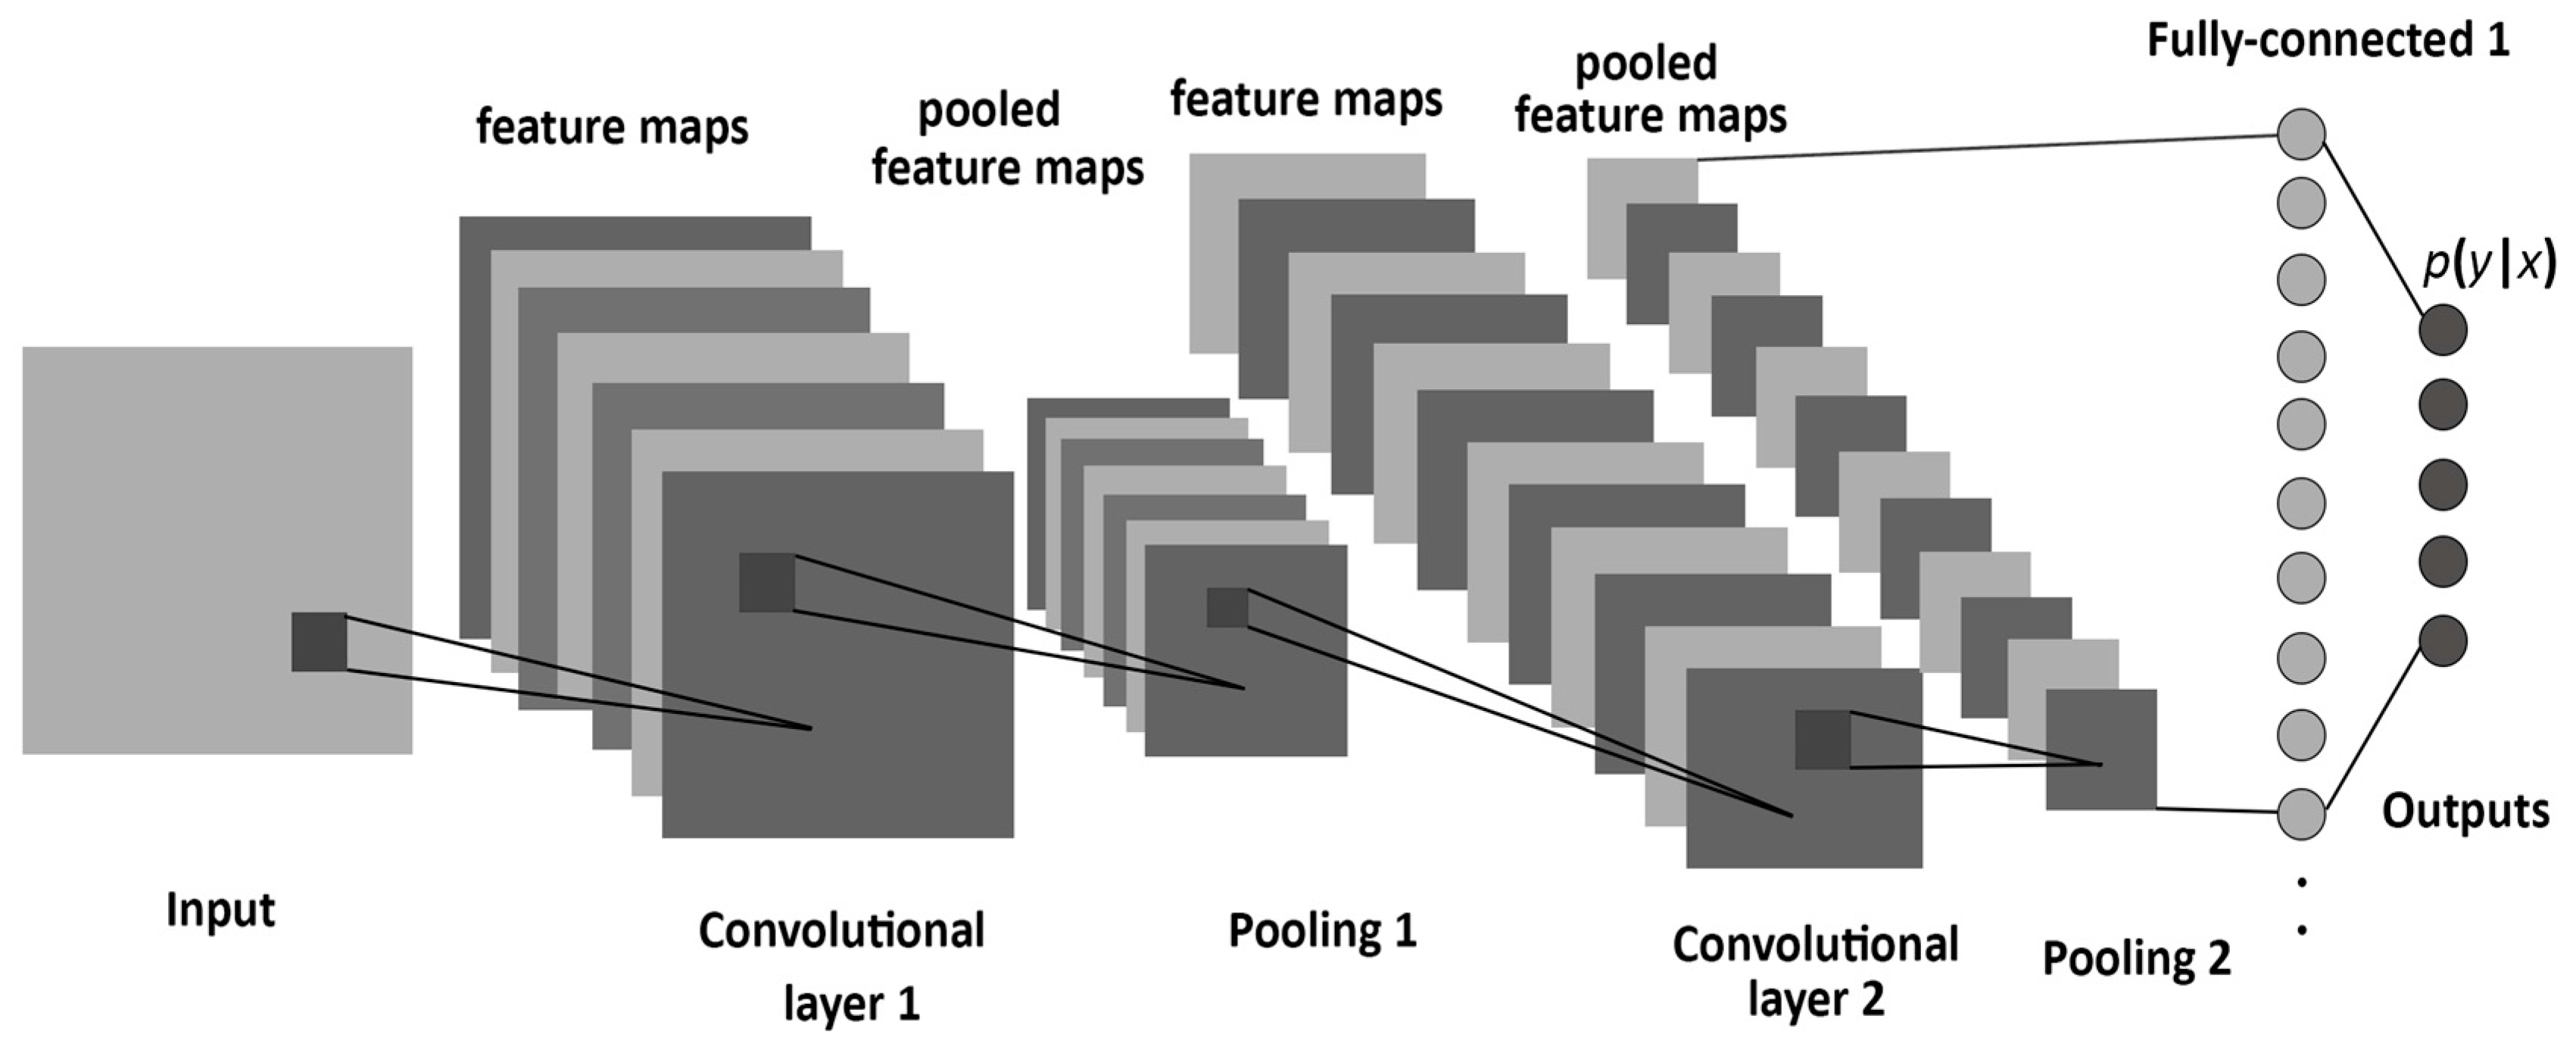
\includegraphics[width=0.8\linewidth]{figures/cnn}
  \caption{A diagram of the basic structure of the network.}
\end{figure}

\subsection{Convolutional Layers}

Each convolutional layer applied a number of convolution filters to 5x5 subregions of the image. This forced the neural network to consider regions of the image in the same way a human might from its start, instead of allowing it to learn that groups of nearby pixels have significance over many training steps.

The first convolutional layer applied 16 filters, which multiplied the size of the data by 16. The second applied 32 filters, which similarly increased the size by 32.

The second convolutional layer was acting not on pixels, but on the data generated by the first convolutional layer. Essentially, it drew inferences about the input not from relationships between groups of pixels, but from relationships between groups of those groups.

\subsection{Pooling Layers}

Between the two convolutional layers, the amount of data being processed grows massively, which greatly increases the amount of processing time required for training. This was remedied in part by the inclusion of pooling layers after each convolutional layer, which reduced the resolution of the data by a factor of four. This comes at a cost to quality of classification, but with such a great decrease in processing time, its inclusion is well worth it.

The specific method of pooling used was max pooling over 2x2 regions with a step size of 2. This means that the data entering the layer was broken into discrete 2x2 regions, and each was reduced to its single highest value. Another method, such as taking the average of the values within each region, or taking the most extreme value coud have been used. This process can be thought of in much the same way one can think of reducing the resolution on any image. Quality is indisputably lost, but without massive reduction in resolution, the image is still much the same.

\subsection{Dense Layer}

Finally, after all convolution and pooling is complete, the data passes through one dense, or fully connnected layer, which simply draws patterns from the data passed in, which is finally reduced to ten values, one for each possible label. The greatest output value acts as the network's prediction. The specific dense layer used here contained 512 nodes.

This layer had a dropout rate of 40\%, which means that 40\% of values, randomly selected, are simply not passed forwards. This encourages a robustness in the network that should allow it to succeed at classification even missing 40\% of data, and should help to avoid total reliance on any one feature.

\subsection{Activation Functions}

Both the convolutional and dense layers use the ReLU activation function:

\begin{equation*}
	f(x) = \max(0, x)
\end{equation*}

This serves to normalize the outputs of each layer. This process has strong biological motivations and mathematical justifications, and has been shown to enable better training of neural networks (Hahnloser, et al. (2013)).

\section{Training}

In order to train the network, a batch of randomly selected training samples is selected and run through the network. Outputs are generated by the network for each member of the batch, and loss is calculated. Loss is simply the difference between the desired output and the actual output of the network. In this case, the desired output is a zero for each label except for the correct one, which should have a value of one.

This loss is used to perform gradient descent on the network, by which weight values are changed from the output layer working back towards the beginning, such that, should the same input arrive again, the actual output will be closer to the desired output. The learning rate for this process was selected as 0.001. This value was selected arbitrarily, and could very well be changed for better results. Empirical testing is required to find the best learning rate.

\begin{figure}
  \centering
  	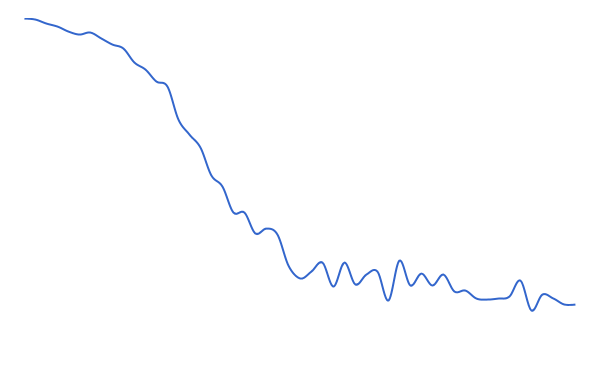
\includegraphics[width=0.8\linewidth]{figures/chart}
  \caption{Change in loss over the course of the training.}
\end{figure}

As can be seen in figure 3, reduction in loss started to diminish near the end of training. This indicates that simply performing additional training would see diminishing returns, and that, to improve the accuracy of the network, there would have to be changes in design.

This process was repeated 5000 times, and then the network was reset, and learning was done again from scratch twice more.

\subsection{Stochastic Gradient Descent}

Stochastic gradient descent is the process by which weights between nodes within the network are modified to improve the accuracy of the network. Starting at the last layer of the network, and working towards the front, weights are changed based on the following equation:

\begin{equation*}
	w = w - \eta \nabla Q(w) = w - \eta \sum_{i=1}^{n} \nabla Q_i(w)/n
\end{equation*}

Where $w$ is the weight of a node, $\eta$ is the learning rate, and $Q(w)$ is the error to be minimized.

\section{Results}

Training steps took on average 27.3 seconds each. The average accuracy after training was 93.55\%. Compared to some attempts at solving the same problem with neural networks, this was a bit of a bust. As of 2013, some attempts were seeing accuracy as high as 99.79\% (Wan, et al. (2013)). Very impressive. With much more training time and number fiddling based on empirical testing, the implimentation described here could possibly have reached similar quality.

\section*{References}

[1] Wan, Li\ \& Zeiler, Matthew\ \& Zhang, Sixin\ \& LeCun, Yann\ \& Fergus, Rob\ (2013) {\it Regularization of Neural Networks using DropConnect}. Dept. of Computer Science, Courant Institute of Mathematical Science, New York University.

[2] R Hahnloser\ \& R. Sarpeshkar\ \& M A Mahowald\ \& R.J. Douglas\ \& H.S. Seung\ (2000) {\it Digital selection and analogue amplification coexist in a cortex-inspired silicon circuit. Nature}. 405. pp. 947-951.

\end{document}
